
\documentclass[french,c,% 't' (resp. 'c') places text vertically at top/center of the slides
% PDF settings
hyperref={%
    pdftitle={Rappels COVID-19},%
    pdfauthor={Guillaume MULLER},%
    pdfsubject={COVID-19},%
    pdfkeywords={COVID-19}%
    colorlinks=true,%
    urlcolor=blue,%
    linkcolor=%
      },%
xcolor={pdftex,svgnames}, % dvipsnames, dvipsnames*, svgnames, svgnames*, x11names,
]{beamer}  %
\usetheme{Copenhagen} % AnnArbor,Antibes,Bergen,Berkeley,Berlin,Boadilla,CambridgeUS,Copenhagen,Darmstadt,Dresden,Frankfurt,Goettingen,Hannover,Ilmenau,JuanLesPins,Luebeck,Madrid,Malmoe,Marburg,Montpellier,PaloAlto,Pittsburgh,Rochester,Singapore,Szeged,Warsaw,boxes,default

% Correct French/English indentation and splitting of words
\usepackage{babel}

% Correct management of accentuated chars in input file
\usepackage[utf8]{inputenc}
%\usepackage[utf8]{inputenc}

% Correct font for the generation of docs with accentuated chars
\usepackage[T1]{fontenc}      % Can handle hyphenation of words with accented characters

% Insertion of images generated by external tools
\usepackage{graphicx}


% Remove navigation bar
%\beamertemplatenavigationsymbolsempty
\setbeamertemplate{navigation symbols}{}
% Remove outline at top
\setbeamertemplate{headline}{}


%%%%%%%%%%%%%%%%%%%%%%%%%%%%%%%%%%%%%%%%%%%%%%%%%%%%%%%%%%%%%%%%%%%%%%
\begin{document}


%%%%%%%%%%%%%%%%%%%%%%%%%%%%%%%%%%%%%%%%
% First slide
\begin{frame}{Rappels COVID-19}
  \begin{itemize}
    \item[] \raisebox{-.45\height}{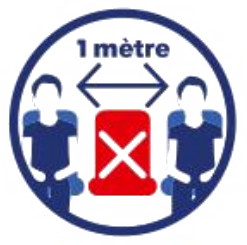
\includegraphics[width=4em]{images00a/distance.png}} \hspace{.8cm}
      Garder les \textbf{distances} { \scriptsize ($>$1~m) }
    \item[] \raisebox{-.45\height}{
\includegraphics[width=4em]{images00a/lavage_mains.png}} \hspace{.8cm}
      Se laver régulièrement les \textbf{mains} { \scriptsize ($\approx$30 min.) }
    \item[] \raisebox{-.45\height}{
\includegraphics[width=4em]{images00a/masque.png}} \hspace{.8cm}
      Mettre un \textbf{masque} { \scriptsize (intérieur+dense, \textbf{nez}+bouche) }
    \item[] \raisebox{-.45\height}{
\includegraphics[width=4em]{images00a/windows10.png}} \hspace{.8cm}
      Ouvrir les \textbf{fenêtres} régulièrement { \scriptsize ($\approx$3 hr.)}
  \end{itemize}
\end{frame}
%%%%%%%%%%%%%%%%%%%%%%%%%%%%%%%%%%%%%%%%


\end{document}


%%% Local Variables:
%%% mode: latex
%%% TeX-master: t
%%% End:
